\subsection{Shape Initialization}\label{sec:initialization}

\cxj{re-write this section. Describe clearly about the parameters, the objective, and methods. }

In this section we explain the reason why using a specific angle to each fold edge, and constructing our initialized model. The basic ideal is to interpret the folded state of a box as a series of rotation angles along each edge, and by setting specific value of angles which is $\pi/2$, we can have a rough model to assist the later optimization.
		
Observed from existing data in the Internet, most of the traditional cartons are cuboid to put in files or delivering daily supplies. Although there is a recent trend to design more complicated layouts to attract consumers, the shape of these unusual cartons is similar to orthogonality boxes as their functions are still packaging commodity. 

%Based on the observation above, we set $\pi/2$ as the value of rotation angle to each fold edge, and have the initialized model as Figure~\ref{fig:initial}.

{\color{blue}{Based on the observation above, we decide to set $\pi/2$ as the value of rotation angle to each fold edge. First, the face adjacent graph of a layout is shown in Figure~\ref{fig:midresult} (a)} where each face is a node. and if two faces are connected through a fold edge. Then by regarding the face with maximum area as fixed face, our system breadth first searches its adjacent faces and rotate the adjacent faces around the current node with $\pi/2$, and finally the initialization result has been generated as Figure~\ref{fig:midresult} (e).} 

\begin{figure}[ht]
	\centering
	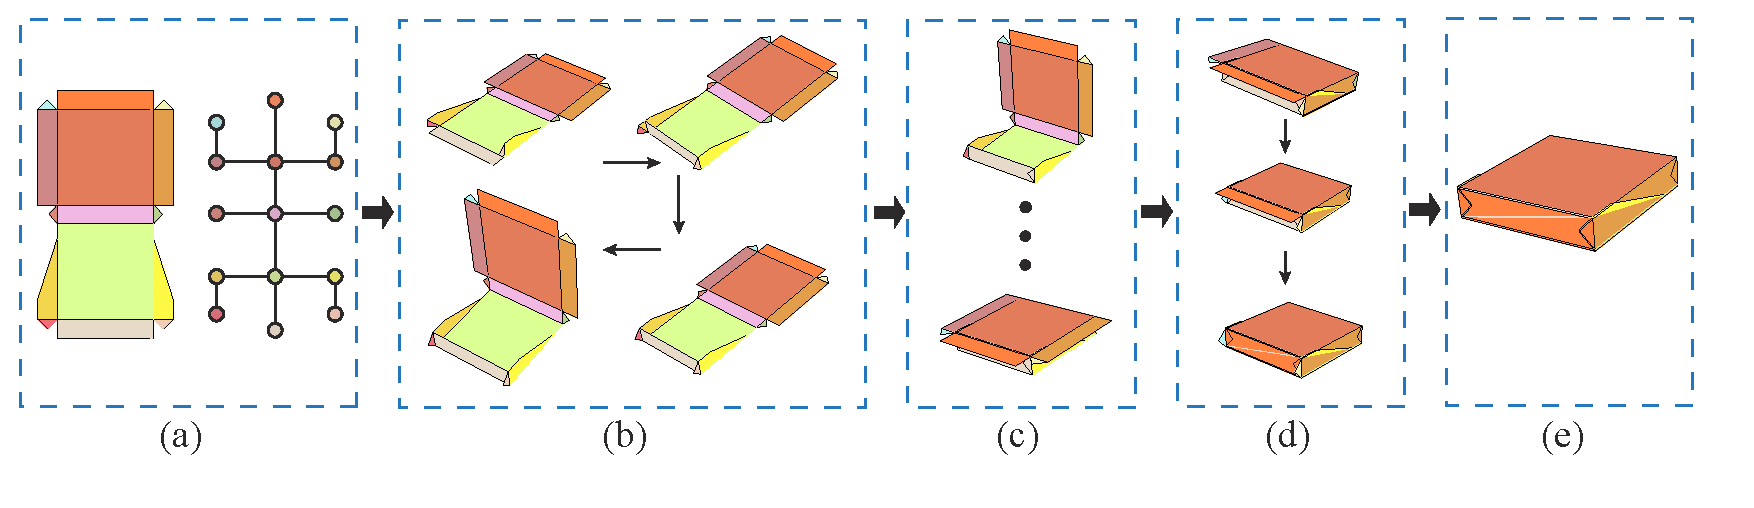
\includegraphics[width=0.9\textwidth]{images/midresult}
	\caption{The folding process of initialization is based on breadth first search the adjacent face start from the face with maximum area. The face adjacent graph of a layout (a) can be obtained by regarding each face as a node, and there is an edge between two nodes if they are connected through a fold edge. (b), (c), (d) and (e) are the different folding stage in initialization.}
	\label{fig:midresult}
\end{figure}

As shown in Figure~\ref{fig:initial} (a), the traditional cartons as cuboid boxes can reach an ideal state, while the novel designs need a little refinement like the four examples in Figure~\ref{fig:initial} (b). Take the hexagonal box as an example, users only need to assign six paste faces into corresponding surface, then the model of a feasible carton will be generated. As a result, we interactively allow users to add these constrains into our system and optimize to a desired model, as described in the following section.

\begin{figure}
	\centering
	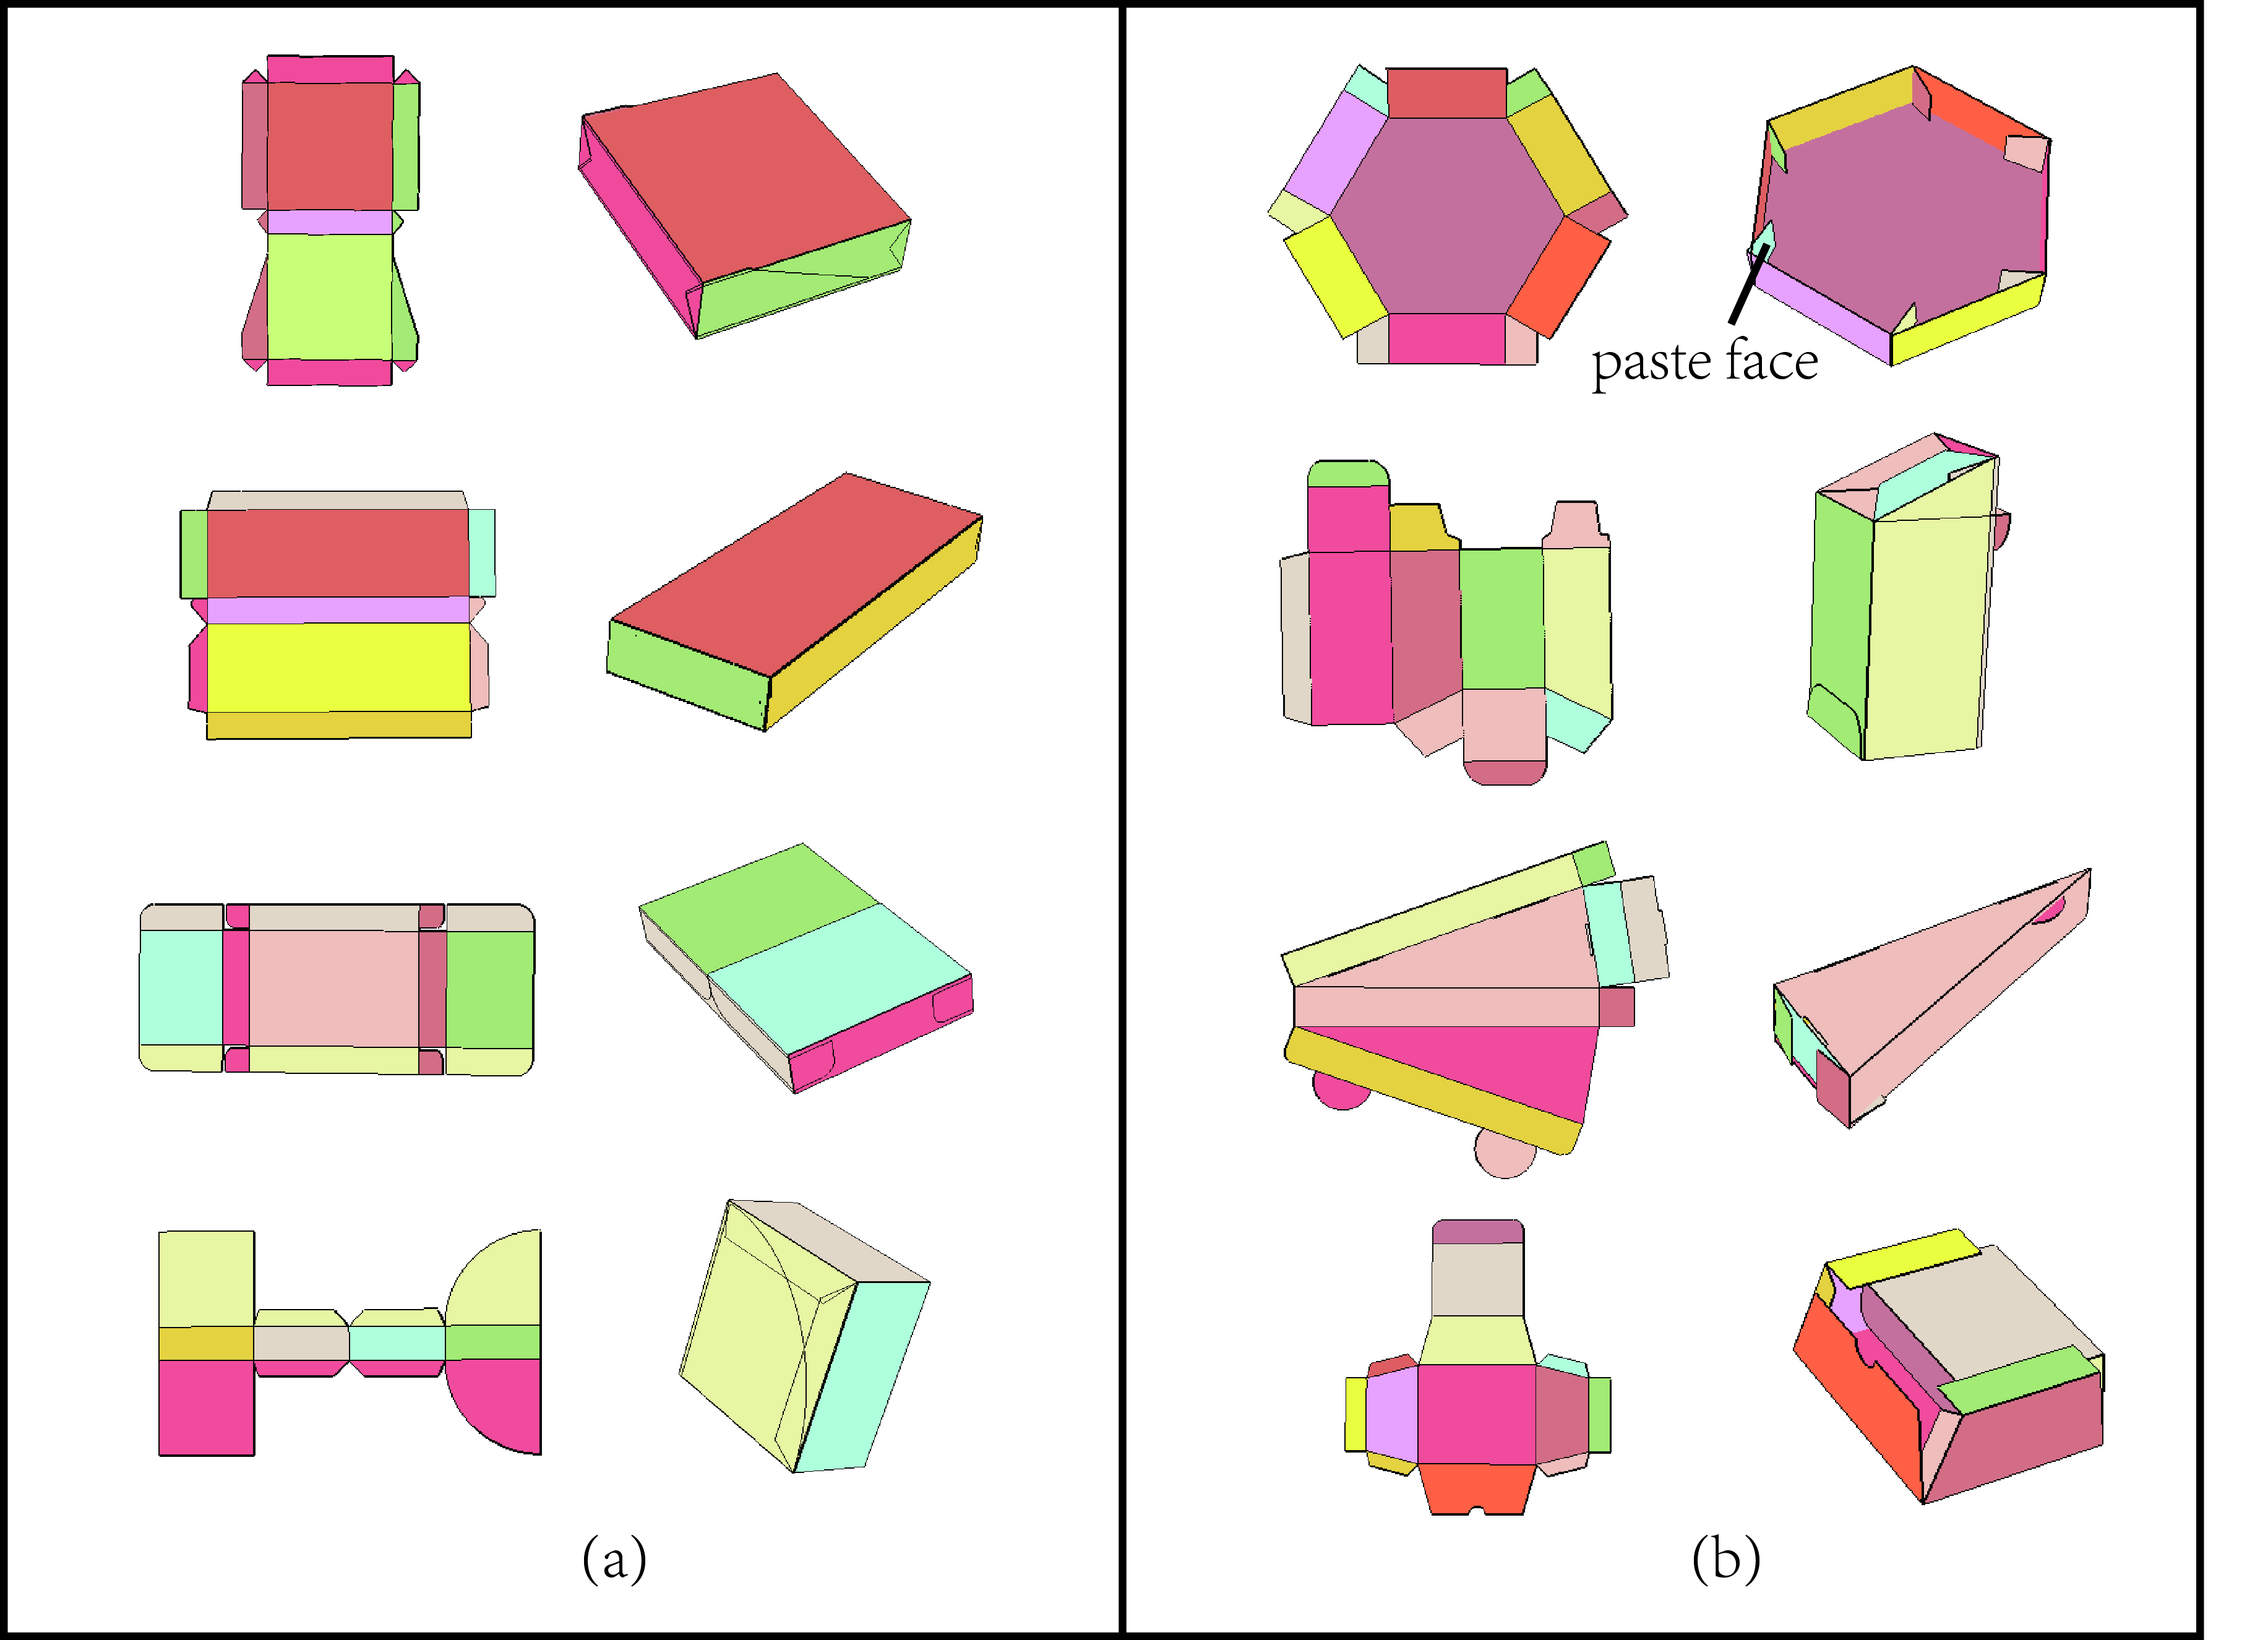
\includegraphics[width=0.9\textwidth]{images/initial.jpg}
	\caption{Eight different initialization results. Four initial cartons shown in the second column of (a) can reach the ideal state, the other four cartons need further refine (b).}
	\label{fig:initial}
\end{figure}

%%%%%%%%%%%%%%%%%%%%%%%%%%%%%%%%%%%%%%%%%%%%%%%%%%%%%%%%%%%%%%%%%%%%%
